\documentclass[journal,10pt,twocolumn]{article}
\usepackage{graphicx}
\usepackage{commath}
\usepackage{gensymb}
\usepackage{caption} 
\usepackage{hyperref}
\usepackage[margin=0.5in]{geometry}
\usepackage{booktabs}
\usepackage{array}
\usepackage{amsmath}   % for having text in math mode
\usepackage{mathtools}
\usepackage{enumitem}
\usepackage{atbegshi}% http://ctan.org/pkg/atbegshi
\AtBeginDocument{\AtBeginShipoutNext{\AtBeginShipoutDiscard}}
\newcommand{\myvec}[1]{\ensuremath{\begin{pmatrix}#1\end{pmatrix}}}
\let\vec\mathbf
\newcommand{\mydet}[1]{\ensuremath{\begin{vmatrix}#1\end{vmatrix}}}
\providecommand{\brak}[1]{\ensuremath{\left(#1\right)}}
\newcommand{\solution}{\noindent \textbf{Solution: }}
\let\vec\mathbf
\begin{document}
\begin{center}
\title{\textbf{Properties of vectors}}
\date{\vspace{-5ex}} %Not to print date automatically
\maketitle
\end{center}
\setcounter{page}{1}
\section{12$^{th}$ Maths - Exercise 10.4.1}

\begin{enumerate}
\item Find $\abs{\overrightarrow{a}\times\overrightarrow{b}}\text{ if }\overrightarrow{a}=\hat{i}-7\hat{j}+7\hat{k}\text{ and }\overrightarrow{b}=3\hat{i}-2\hat{j}+2\hat{k}$
\section{Solution}
Now,
\begin{align}
\overrightarrow{a}\times \overrightarrow{b} &=\begin{vmatrix}
i & j & k\\
1 & -7 & 7\\
3 & -2 & 2
\end{vmatrix}\\
&=0\hat{i}+19\hat{j}+19\hat{k}
\end{align}
Therefore
\begin{align}
\abs{\overrightarrow{a}\times \overrightarrow{b}}&=\sqrt{0^2+19^2+19^2}\\
\implies 26.87
\end{align}
\begin{figure}[h]
	  \centering 
	  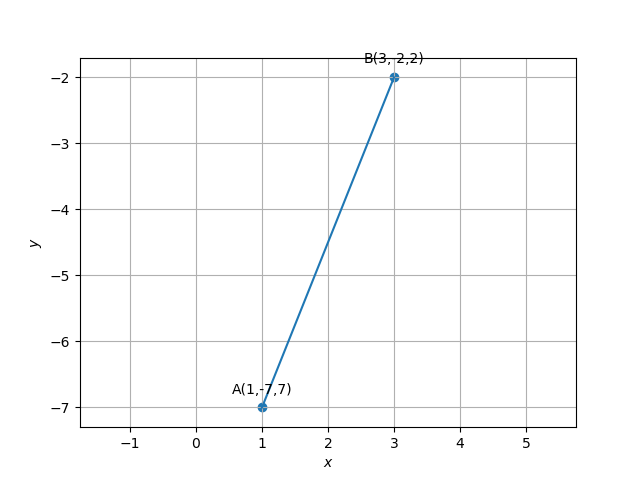
\includegraphics[width=\columnwidth]{nom.png}
	  \caption{}
	  \label{fig:nom.png}
	  \end{figure}
\end{enumerate}
\end{document}